\documentclass[11pt,aspectratio=169]{beamer}
\usepackage{amsmath,amssymb,bm,booktabs,tikz}
\usetikzlibrary{arrows.meta,calc}
\usetheme{default}
\setbeamertemplate{navigation symbols}{}
\setbeamertemplate{headline}{}
\setbeamertemplate{footline}{%
  \leavevmode\hbox{%
    \begin{beamercolorbox}[wd=\paperwidth,ht=2.6ex,dp=1.1ex,right]{page number in head/foot}%
      \insertframenumber/\inserttotalframenumber\hspace{0.35cm}
    \end{beamercolorbox}}}
\setbeamertemplate{frametitle}{\vspace{0.25cm}\insertframetitle\par\vspace{0.08cm}\hrule}
\setbeamercolor{normal text}{fg=black,bg=white}
\setbeamercolor{frametitle}{fg=black,bg=white}
\setbeamercolor{structure}{fg=black}
\setbeamersize{text margin left=0.7cm,text margin right=0.7cm}
\definecolor{femblue}{RGB}{47,99,143}
\definecolor{femorange}{RGB}{198,91,42}
\definecolor{femgreen}{RGB}{39,117,83}
\newcommand{\bu}{\bm u}
\newcommand{\bv}{\bm v}
\newcommand{\bw}{\bm w}
\newcommand{\bx}{\bm x}
\newcommand{\bX}{\bm X}
\newcommand{\bn}{\bm n}
\newcommand{\bN}{\bm N}
\newcommand{\bb}{\bm b}
\newcommand{\bt}{\bm t}
\newcommand{\bI}{\bm I}
\newcommand{\bF}{\bm F}
\newcommand{\bC}{\bm C}
\newcommand{\bE}{\bm E}
\newcommand{\bP}{\bm P}
\newcommand{\bsig}{\bm\sigma}
\newcommand{\beps}{\bm\varepsilon}
\newcommand{\bphi}{\bm\varphi}
\newcommand{\Grad}{\operatorname{Grad}}
\newcommand{\Div}{\operatorname{Div}}
\newcommand{\divg}{\nabla_{\bx}\!\cdot}
\newcommand{\dd}{\,\mathrm d}
\newcommand{\Vzero}{\mathcal V_0}
\DeclareMathOperator{\tr}{tr}
\DeclareMathOperator{\diag}{diag}

\begin{document}

\begin{frame}
\centering\vfill
{\LARGE\bfseries Nonlinear Finite Element Methods\par}
\vspace{0.5cm}
{\Large Lecture 1: Large Deformation and Reference Formulation\par}
\vspace{0.5cm}
Prashant K. Jha\par
ME/BME 736\par
October 29, 2026
\vfill
\end{frame}

\begin{frame}{Lecture outline}
\begin{enumerate}
\item The difficulty: equilibrium on an unknown deformed body.
\item The deformation map and the geometry needed to describe that body.
\item Mapping surface forces and equilibrium to the reference body.
\item The resulting hyperelastic boundary-value problem.
\end{enumerate}
\vspace{0.3cm}
The closing section develops the variational problem and introduces
Newton's method through a scalar equation.
\end{frame}

\begin{frame}{The loaded body and its unknown shape}
The reference body, its supports, and its applied load are given.
The displacement determines the current shape.
\begin{center}
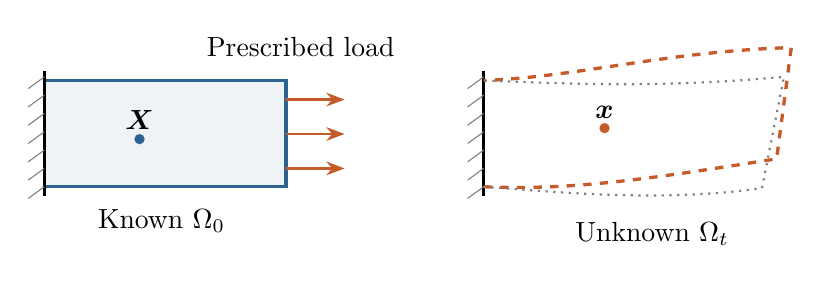
\begin{tikzpicture}[>=Stealth,scale=.93]
\filldraw[draw=femblue,fill=femblue!8,very thick] (0,0) rectangle(3.3,1.45);
\draw[very thick] (0,-.12)--(0,1.58);
\foreach \y in {0,.25,.5,.75,1,1.25,1.5}
  \draw[gray] (0,\y)--(-.22,{\y-.16});
\foreach \y in {.25,.72,1.19}
  \draw[->,thick,femorange] (3.3,\y)--(4.1,\y);
\node[above] at (3.5,1.65) {Prescribed load};
\fill[femblue] (1.3,.65) circle(2pt);
\node[above] at (1.3,.65) {$\bX$};
\node[below] at (1.6,-.18) {Known $\Omega_0$};
\draw[very thick] (6,-.12)--(6,1.58);
\foreach \y in {0,.25,.5,.75,1,1.25,1.5}
  \draw[gray] (6,\y)--(5.78,{\y-.16});
\draw[very thick,dashed,femorange]
  (6,0)..controls(7.3,-.06)and(8.5,.15)..(10,.38)
  --(10.2,1.9)..controls(8.5,1.85)and(7.3,1.5)..(6,1.45);
\draw[dotted,gray,thick]
  (6,0)..controls(7.3,-.1)and(8.5,-.2)..(9.8,-.02)
  --(10.1,1.5)..controls(8.4,1.35)and(7.3,1.4)..(6,1.45);
\fill[femorange] (7.65,.8) circle(2pt);
\node[above] at (7.65,.8) {$\bx$};
\node[below] at (8.3,-.35) {Unknown $\Omega_t$};
\end{tikzpicture}
\end{center}
The dashed and dotted outlines illustrate possible deformed shapes.
Which one satisfies equilibrium must be found.
\end{frame}

\begin{frame}{Equilibrium is written on the current body}
Let $\bsig$ be Cauchy stress, $\bn$ the current outward unit normal,
$\rho$ current density, and $\bb$ body force per unit mass.
Neglect inertia.
\[
-\nabla_{\bx}\!\cdot\bsig=\rho\bb
\quad\text{in }\Omega_t.
\]
For every current material subdomain $\omega_t$, the equivalent force balance is
\[
\boxed{
\int_{\partial\omega_t}\bsig\bn\,\mathrm da
+\int_{\omega_t}\rho\bb\,\mathrm dV_t=\bm0.
}
\]
The domain, its boundary normals and areas, and the stress depend on the
displacement being sought.

We choose a reference formulation so that integration is performed on the
known body $\Omega_0$. Current-configuration formulations are also possible.
\end{frame}

\begin{frame}{The deformation map and its gradient}
Label a material point by $\bX\in\Omega_0$. Its current position is
\[
\bx=\bphi(\bX)=\bX+\bu(\bX).
\]
Taking the total differential of $x_i=\varphi_i(\bX)$ gives
\[
\mathrm dx_i
=\frac{\partial\varphi_i}{\partial X_J}\,\mathrm dX_J
=F_{iJ}\,\mathrm dX_J.
\]
Define the \textbf{deformation gradient}:
\[
\boxed{
\bF=\Grad\bphi=\bI+\Grad\bu,\qquad
\dd\bx=\bF\dd\bX.
}
\]
Here $\Grad$ means differentiation with respect to $\bX$;
$(\Grad\bu)_{iJ}=\partial u_i/\partial X_J$.
Repeated indices are summed.

Assume smooth, one-to-one, orientation-preserving deformations.
\end{frame}

\begin{frame}{Example: local deformation}
In a small material region, consider the following local deformation:
\[
\bx=
\begin{bmatrix}1.5X_1\\0.8X_2\\X_3\end{bmatrix},
\qquad
\bF=\begin{bmatrix}1.5&0&0\\0&0.8&0\\0&0&1\end{bmatrix}.
\]
\begin{center}
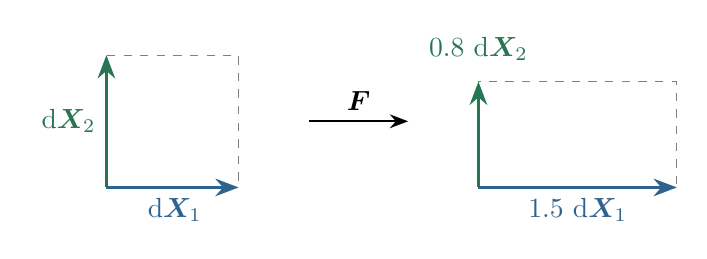
\begin{tikzpicture}[>=Stealth,scale=1.05]
\draw[gray,dashed] (0,0) rectangle(1.6,1.6);
\draw[->,very thick,femblue] (0,0)--(1.6,0)
  node[midway,below] {$\dd\bX_1$};
\draw[->,very thick,femgreen] (0,0)--(0,1.6)
  node[midway,left] {$\dd\bX_2$};
\draw[->,thick] (2.45,.8)--(3.65,.8)
  node[midway,above] {$\bF$};
\draw[gray,dashed] (4.5,0) rectangle(6.9,1.28);
\draw[->,very thick,femblue] (4.5,0)--(6.9,0)
  node[midway,below] {$1.5\,\dd\bX_1$};
\draw[->,very thick,femgreen] (4.5,0)--(4.5,1.28);
\node[femgreen,above] at (4.5,1.42) {$0.8\,\dd\bX_2$};
\end{tikzpicture}
\end{center}
A line parallel to the first axis lengthens by $50\%$.
A line parallel to the second axis shortens by $20\%$.
\end{frame}

\begin{frame}{Measuring deformation: $\bC$ and $\bE$}
The line mapping gives
\[
\dd\bx\cdot\dd\bx
=(\bF\dd\bX)\cdot(\bF\dd\bX)
=\dd\bX\cdot(\bF^T\bF)\dd\bX.
\]
Define the \textbf{right Cauchy--Green tensor} $\bC=\bF^T\bF$.
The change in squared length is
\[
|\dd\bx|^2-|\dd\bX|^2
=\dd\bX\cdot(\bC-\bI)\dd\bX.
\]
The \textbf{Green--Lagrange strain} is therefore
\[
\boxed{
\bE=\tfrac12(\bC-\bI),\qquad
|\dd\bx|^2-|\dd\bX|^2=2\dd\bX\cdot\bE\dd\bX.
}
\]
For the preceding example,
$C_{11}=1.5^2=2.25$ and $E_{11}=(2.25-1)/2=0.625$.
\end{frame}

\begin{frame}{Why infinitesimal strain is insufficient}
Substitute $\bF=\bI+\Grad\bu$ into $\bE=(\bF^T\bF-\bI)/2$:
\[
\boxed{
\bE=\tfrac12\left(
\Grad\bu+(\Grad\bu)^T+(\Grad\bu)^T\Grad\bu
\right).
}
\]
Infinitesimal strain neglects the last, quadratic term.
That approximation requires a small displacement gradient.
\begin{columns}[c,onlytextwidth]
\begin{column}{.32\textwidth}
\centering
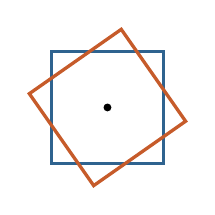
\begin{tikzpicture}[scale=.95]
\draw[very thick,femblue] (-.75,-.75) rectangle(.75,.75);
\draw[very thick,femorange,rotate=35] (-.75,-.75) rectangle(.75,.75);
\fill (0,0) circle(1.5pt);
\end{tikzpicture}
\end{column}
\begin{column}{.65\textwidth}
A rigid rotation changes orientation but not material lengths.
Its deformation gradient satisfies
\[
\bF^T\bF=\bI,\qquad \bE=\bm0.
\]
Retaining the quadratic term makes this check hold even for a large rotation.
\end{column}
\end{columns}
\end{frame}

\begin{frame}{Volume mapping}
Define $J=\det\bF$. Corresponding infinitesimal volumes satisfy
\[
\boxed{\mathrm dV_t=J\,\mathrm dV_0.}
\]
For the same numerical deformation,
\[
J=(1.5)(0.8)(1)=1.2.
\]
A reference material region of volume $1$ has current volume $1.2$.
For any integrable current field $g$,
\[
\boxed{
\int_{\Omega_t}g(\bx)\,\mathrm dV_t
=\int_{\Omega_0}g(\bphi(\bX))J(\bX)\,\mathrm dV_0.
}
\]
We require $J>0$ locally. Together with the assumed one-to-one map, this
allows the change of variables to the reference body.
\end{frame}

\begin{frame}{Surface forces need an area and a normal mapping}
On a current surface patch,
\[
\bt=\bsig\bn,\qquad
\mathrm d\bm f=\bsig\bn\,\mathrm da.
\]
Let $\mathrm dA$ and $\bN$ be the corresponding reference area and outward
unit normal. To express the same force using them, we must map both the area
and its normal.
\begin{center}
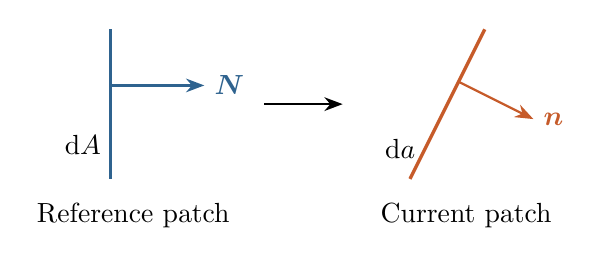
\begin{tikzpicture}[>=Stealth,scale=.95]
\draw[very thick,femblue] (0,0)--(0,2);
\draw[->,thick,femblue] (0,1.25)--(1.25,1.25)
  node[right] {$\bN$};
\node[left] at (0,.45) {$\mathrm dA$};
\node[below] at (.3,-.2) {Reference patch};
\draw[->,thick] (2.05,1)--(3.1,1);
\draw[very thick,femorange] (4,0)--(5,2);
\draw[->,thick,femorange] (4.65,1.3)--(5.65,.8)
  node[right] {$\bn$};
\node[left] at (4.2,.4) {$\mathrm da$};
\node[below] at (4.75,-.2) {Current patch};
\end{tikzpicture}
\end{center}
The surface patches are shown in cross-section.
The general map can change their orientation as well as their area.
\end{frame}

\begin{frame}{Nanson's formula: mapping the oriented area}
Let two reference edge vectors $\bm A$ and $\bm B$ span a small surface patch:
\[
\bN\,\mathrm dA=\bm A\times\bm B.
\]
The corresponding current edges are $\bF\bm A$ and $\bF\bm B$.
Using the cross-product transformation,
\[
\begin{aligned}
\bn\,\mathrm da
&=(\bF\bm A)\times(\bF\bm B)\\
&=J\bF^{-T}(\bm A\times\bm B)\\
&=J\bF^{-T}\bN\,\mathrm dA.
\end{aligned}
\]
Thus \textbf{Nanson's formula} is
\[
\boxed{\bn\,\mathrm da=J\bF^{-T}\bN\,\mathrm dA.}
\]
The vector on the right contains both the current normal direction and
the current area. $\bF^{-T}\bN$ is generally not a unit vector.
\end{frame}

\begin{frame}{First Piola--Kirchhoff stress}
Define the \textbf{first Piola--Kirchhoff stress} $\bP$ by
\[
\mathrm d\bm f=\bP\bN\,\mathrm dA.
\]
Insert Nanson's formula into the current force expression:
\[
\begin{aligned}
\mathrm d\bm f
&=\bsig\bn\,\mathrm da\\
&=\bsig\left(J\bF^{-T}\bN\,\mathrm dA\right)\\
&=\left(J\bsig\bF^{-T}\right)\bN\,\mathrm dA.
\end{aligned}
\]
Therefore
\[
\boxed{\bP=J\bsig\bF^{-T},\qquad
\bsig=\frac1J\bP\bF^T.}
\]
$\bP\bN$ is physical force per unit reference area.
$\bP$ is generally nonsymmetric, even though $\bsig$ is symmetric.
\end{frame}

\begin{frame}{The same force divided by different areas}
For $\bF=\diag(1.5,0.8,1)$, a face normal to the first axis keeps its normal
direction, but its area is multiplied by $0.8$.
\begin{center}
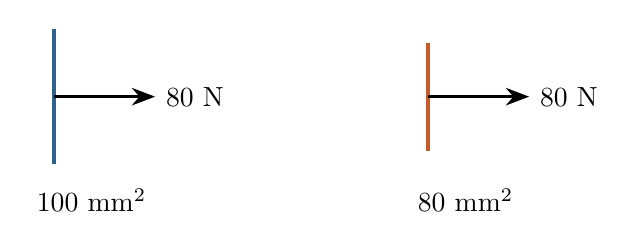
\begin{tikzpicture}[>=Stealth,scale=.95]
\draw[very thick,femblue] (0,0)--(0,1.8);
\draw[->,very thick] (0,.9)--(1.35,.9) node[right] {$80\ \mathrm N$};
\node[below] at (.5,-.2) {$100\ \mathrm{mm}^2$};
\draw[very thick,femorange] (5,.18)--(5,1.62);
\draw[->,very thick] (5,.9)--(6.35,.9) node[right] {$80\ \mathrm N$};
\node[below] at (5.5,-.2) {$80\ \mathrm{mm}^2$};
\end{tikzpicture}
\end{center}
The normal stress values are
\[
P_{11}=\frac{80\ \mathrm N}{100\ \mathrm{mm}^2}=0.8\ \mathrm{MPa},
\qquad
\sigma_{11}=\frac{80\ \mathrm N}{80\ \mathrm{mm}^2}=1\ \mathrm{MPa}.
\]
They agree with $P_{11}=(J/F_{11})\sigma_{11}
=(1.2/1.5)\sigma_{11}$.
The force is unchanged. Only its area basis differs.
\end{frame}

\begin{frame}{Force balance on the reference body}
Return to current equilibrium on $\omega_t=\bphi(\omega_0)$:
\[
\bm0=
\int_{\partial\omega_t}\bsig\bn\,\mathrm da
+\int_{\omega_t}\rho\bb\,\mathrm dV_t.
\]
Use $\bsig\bn\,\mathrm da=\bP\bN\,\mathrm dA$ and
$\mathrm dV_t=J\,\mathrm dV_0$:
\[
\bm0=
\int_{\partial\omega_0}\bP\bN\,\mathrm dA
+\int_{\omega_0}\rho(\bphi(\bX))\bb(\bphi(\bX))J\,\mathrm dV_0.
\]
Define body force per unit reference volume by
\[
\bb_0(\bX)=J(\bX)\rho(\bphi(\bX))\bb(\bphi(\bX)).
\]
The same equilibrium statement is now
\[
\boxed{
\int_{\partial\omega_0}\bP\bN\,\mathrm dA
+\int_{\omega_0}\bb_0\,\mathrm dV_0=\bm0.
}
\]
\end{frame}

\begin{frame}{Current and reference equilibrium}
Apply the reference divergence theorem to the preceding surface integral:
\[
\int_{\omega_0}(\Div\bP+\bb_0)\,\mathrm dV_0=\bm0.
\]
For arbitrary $\omega_0$, with sufficiently regular fields, this gives
\[
\begin{array}{c@{\qquad\qquad}c}
\text{Current body}&\text{Reference body}\\[.3em]
-\nabla_{\bx}\!\cdot\bsig=\rho\bb
&
-\Div\bP=\bb_0\\[.3em]
\bx\in\Omega_t
&
\bX\in\Omega_0
\end{array}
\]
The operators use different coordinates:
\[
(\nabla_{\bx}\!\cdot\bsig)_i
=\frac{\partial\sigma_{ij}}{\partial x_j},
\qquad
(\Div\bP)_i=\frac{\partial P_{iJ}}{\partial X_J}.
\]
These are descriptions of the same force balance, not different physical models.
\end{frame}

\begin{frame}{Boundary data must use the corresponding area}
Partition the reference boundary into $\Gamma_{0u}$ and $\Gamma_{0t}$:
\[
\bu=\overline{\bu}\quad\text{on }\Gamma_{0u},
\qquad
\bP\bN=\overline{\bt}_0\quad\text{on }\Gamma_{0t}.
\]
On the corresponding current traction boundary
$\Gamma_{tt}=\bphi(\Gamma_{0t})$,
\[
\bsig\bn=\overline{\bt}.
\]
The prescribed tractions represent the same force when
\[
\boxed{
\overline{\bt}_0\,\mathrm dA
=\overline{\bt}\,\mathrm da.
}
\]
For our loaded body, prescribe both $\overline{\bt}_0$ per reference area
and $\bb_0$ per reference volume independently of displacement.

Holding a traction per reference area fixed is generally different from
holding its current-area value fixed while the surface changes.
\end{frame}

\begin{frame}{Hyperelastic stress law}
A hyperelastic material supplies stored energy per reference volume,
$\Psi(\bF)$, and the stress law
\[
\bP=\frac{\partial\Psi}{\partial\bF}.
\]
Recall the compressible neo-Hookean model from Chapter 4:
\[
\Psi(\bF)
=\frac\mu2(\tr(\bF^T\bF)-3)
-\mu\ln J+\frac\lambda2(\ln J)^2,
\qquad J>0.
\]
Its first Piola--Kirchhoff stress is
\[
\boxed{\bP(\bF)
=\mu(\bF-\bF^{-T})+\lambda\ln J\,\bF^{-T}.}
\]
Here $\mu$ and $\lambda$ are the material's Lam\'e constants.
The stress depends on $\bu$ through $\bF=\bI+\Grad\bu$,
including its inverse and determinant.
\end{frame}

\begin{frame}{Reference-configuration strong problem}
With $\bF(\bu)=\bI+\Grad\bu$, the problem is
\[
\left\{\begin{aligned}
-\Div\bP(\bF(\bu))&=\bb_0&&\text{in }\Omega_0,\\
\bu&=\overline{\bu}&&\text{on }\Gamma_{0u},\\
\bP(\bF(\bu))\bN&=\overline{\bt}_0&&\text{on }\Gamma_{0t}.
\end{aligned}\right.
\qquad\text{Strong form}
\]
The reference mesh, integration domain, and material labels are known.

The deformation and stress remain unknown. For the neo-Hookean law,
$\bF^{-T}$ and $\ln(\det\bF)$ depend nonlinearly on $\Grad\bu$.

A guessed displacement lets us evaluate the stress, but that stress generally
does not satisfy equilibrium. The displacement must be corrected.
\end{frame}

\begin{frame}{Trial and test functions on the known reference body}
Use the Chapter 4 trial and test spaces:
\[
\begin{aligned}
\mathcal U_{\overline{\bu}}
&=\{\bw\in H^1(\Omega_0;\mathbb R^3):
\bw=\overline{\bu}\text{ on }\Gamma_{0u}\},\\
\Vzero
&=\{\bv\in H^1(\Omega_0;\mathbb R^3):
\bv=\bm0\text{ on }\Gamma_{0u}\}.
\end{aligned}
\]
Assume admissible deformations with $J>0$ and enough regularity for the
following stress integrals to be finite.
For $\bv\in\Vzero$, start with $-\Div\bP=\bb_0$:
\[
-\int_{\Omega_0}(\Div\bP)\cdot\bv\,\mathrm dV_0
=\int_{\Omega_0}\bb_0\cdot\bv\,\mathrm dV_0.
\]
The unknown and test functions are defined using the fixed coordinates $\bX$.
\end{frame}

\begin{frame}{Reference-domain variational problem}
Integration by parts in the preceding equation gives
\[
\int_{\Omega_0}\bP:\Grad\bv\,\mathrm dV_0
-\int_{\partial\Omega_0}(\bP\bN)\cdot\bv\,\mathrm dA
=\int_{\Omega_0}\bb_0\cdot\bv\,\mathrm dV_0.
\]
On $\Gamma_{0u}$, $\bv=\bm0$. On $\Gamma_{0t}$,
$\bP\bN=\overline{\bt}_0$. Substituting these conditions gives
\[
\begin{aligned}
\int_{\Omega_0}\bP(\bF(\bu)):\Grad\bv\,\mathrm dV_0
={}&\int_{\Omega_0}\bb_0\cdot\bv\,\mathrm dV_0\\
&+\int_{\Gamma_{0t}}\overline{\bt}_0\cdot\bv\,\mathrm dA.
\end{aligned}
\]
Find $\bu\in\mathcal U_{\overline{\bu}}$ such that this holds for every
$\bv\in\Vzero$.

The gradient is $\Grad\bv$, not its symmetric part, because $\bP$ is
generally nonsymmetric.
\end{frame}

\begin{frame}{Why the finite element equations are nonlinear}
Write the internal form and external load functional as
\[
\begin{aligned}
a_{\mathrm{hyp}}(\bu;\bv)
&=\int_{\Omega_0}\bP(\bF(\bu)):\Grad\bv\,\mathrm dV_0,\\
\ell_{\mathrm{hyp}}(\bv)
&=\int_{\Omega_0}\bb_0\cdot\bv\,\mathrm dV_0
+\int_{\Gamma_{0t}}\overline{\bt}_0\cdot\bv\,\mathrm dA.
\end{aligned}
\]
The residual is
\[
\boxed{R(\bu;\bv)=\ell_{\mathrm{hyp}}(\bv)-a_{\mathrm{hyp}}(\bu;\bv).}
\]
Equilibrium requires $R(\bu;\bv)=0$ for every test function.

After FE approximation, the stress depends on the unknown displacement
coefficients. We must solve nonlinear equations for those coefficients,
rather than one system with a fixed stiffness matrix.
\end{frame}

\begin{frame}{Newton's method: one scalar equation}
Consider $r(z)=z^2-2=0$. Let $z^k$ be an approximation and
$\Delta z^k$ its correction.
Linearize about $z^k$:
\[
r(z^k+\Delta z^k)
\approx r(z^k)+r'(z^k)\Delta z^k.
\]
Set this linear approximation to zero:
\[
\boxed{r'(z^k)\Delta z^k=-r(z^k),\qquad
z^{k+1}=z^k+\Delta z^k.}
\]
Starting from $z^0=1$,
\[
r(1)=-1,\qquad r'(1)=2,\qquad
2\Delta z^0=1,\qquad z^1=1.5.
\]
Each iteration solves a linear correction equation and updates the approximation.
\end{frame}

\begin{frame}{A tangent equation predicts the next approximation}
\begin{columns}[c,onlytextwidth]
\begin{column}{.62\textwidth}
\centering
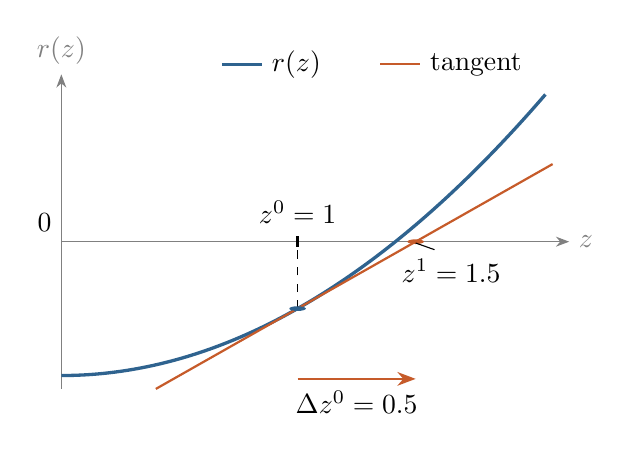
\begin{tikzpicture}[>=Stealth,xscale=3,yscale=.85]
\draw[->,gray] (0,0)--(2.15,0) node[right] {$z$};
\draw[->,gray] (0,-2.2)--(0,2.5) node[above] {$r(z)$};
\node[above left] at (0,0) {$0$};
\draw[very thick,femblue,domain=0:2.05,samples=90]
  plot(\x,{\x*\x-2});
\draw[thick,femorange,domain=.4:2.08] plot(\x,{2*\x-3});
\draw[dashed] (1,-1)--(1,0);
\fill[femblue] (1,-1) circle(1pt);
\draw[thick] (1,.08)--(1,-.08);
\node[above] at (1,.12) {$z^0=1$};
\fill[femorange] (1.5,0) circle(1pt);
\node[below] at (1.65,-.12) {$z^1=1.5$};
\draw[thin] (1.5,-.02)--(1.58,-.12);
\draw[->,femorange,thick] (1,-2.05)--(1.5,-2.05);
\node[below] at (1.25,-2.08) {$\Delta z^0=0.5$};
\draw[very thick,femblue] (.68,2.65)--(.85,2.65);
\node[right] at (.85,2.65) {$r(z)$};
\draw[thick,femorange] (1.35,2.65)--(1.52,2.65);
\node[right] at (1.52,2.65) {tangent};
\end{tikzpicture}
\end{column}
\begin{column}{.35\textwidth}
The tangent at $z^0=1$ is
\[
r(1)+r'(1)(z-1)=2z-3.
\]
Its zero gives $z^1=1.5$.

Repeating the update gives
\[
1.5,\quad1.416667,\quad1.414216.
\]
The tangent must be evaluated again at each new iterate.
\end{column}
\end{columns}
\end{frame}

\begin{frame}{The same correction idea for displacement}
For hyperelasticity, seek $R(\bu;\bv)=0$ for every $\bv\in\Vzero$.
Hold $\bv$ fixed and define the directional derivative
\[
D_uR(\bu;\bv)[\bw]
=\left.\frac{\mathrm d}{\mathrm d\epsilon}
R(\bu+\epsilon\bw;\bv)\right|_{\epsilon=0}.
\]
The first-order expansion is
\[
R(\bu^k+\Delta\bu^k;\bv)
\approx R(\bu^k;\bv)+D_uR(\bu^k;\bv)[\Delta\bu^k].
\]
Setting this approximation to zero gives the linear correction problem
\[
\boxed{D_uR(\bu^k;\bv)[\Delta\bu^k]
=-R(\bu^k;\bv)\quad\forall\bv\in\Vzero.}
\]
Update $\bu^{k+1}=\bu^k+\Delta\bu^k$.
If the iterate satisfies the prescribed displacement, the correction is zero
on $\Gamma_{0u}$. The next lecture constructs this tangent problem explicitly.
\end{frame}

\begin{frame}{Summary and next step}
\begin{itemize}
\item Large deformation changes the body on which equilibrium is written.
We choose a known reference domain for the FE formulation.
\item The deformation gradient maps line elements.
Its determinant maps volume. Nanson's formula maps oriented surface area.
\item Preserving physical force gives $\bP=J\bsig\bF^{-T}$ and
reference equilibrium $-\Div\bP=\bb_0$.
\item Mapping fixes the integration domain, but does not make
$\bP(\bI+\Grad\bu)$ linear in displacement.
\end{itemize}
The next step is to linearize the residual and assemble the Newton correction
system for the hyperelastic FE problem.
\end{frame}

\begin{frame}{Reading and stress convention}
\begin{itemize}
\item Course book, Chapter 4, \emph{Finite deformation and hyperelasticity}:
the material model and reference variational problem used here.
\item Local Belytschko notes, Chapter 2, \S2.2:
material coordinates and the reference-area description of force.
\item Local Belytschko notes, Chapter 3, \S3.2--3.4:
deformation gradient, Green strain, and surface/stress transformations.
Nanson's relation appears in \S3.4.2, printed p.\ 3-33.
\item Local Belytschko notes, Chapter 6, \S6.3.3--6.3.4:
Newton's method.
\end{itemize}
Our convention is $\bt_0=\bP\bN$ and $\bP=J\bsig\bF^{-T}$.
The local notes' nominal stress uses the transpose convention.
All formulas in these slides follow the course book.
\end{frame}

\end{document}
